\subsection{BÀI TẬP TRẮC NGHIỆM}
\ind{PHẦN I.} \inden{Câu trắc nghiệm nhiều phương án lựa chọn. Mỗi câu hỏi học sinh chỉ chọn một phương án.}\\
\setcounter{ex}{0}
\Opensolutionfile{ans}[ans/1H7-B3-1]

\begin{ex}
	Cho hình chóp ${S.ABC}$ có đáy là tam giác vuông cân tại ${C}$, $SA\bot (ABC)$. Gọi ${P}$ là trung điểm của cạnh ${AB}$.Gọi ${Q}$ là trung điểm của cạnh ${AC}$. Tìm hình chiếu của điểm ${C}$ trên mặt phẳng $(SAB)$?	
	\choice
	{ Điểm ${S}$ }
	{ Điểm ${Q}$ }
	{ Điểm ${A}$ }
	{ \True Điểm ${P}$ }
	\loigiai{ 
		$CP\bot AB,CP\bot SA \Rightarrow CP\bot (SAB)$. Do đó hình chiếu của điểm ${C}$ trên mặt phẳng $(SAB)$ là điểm ${P}$. 
}\end{ex}

\begin{ex}
	Cho hình chóp ${S.ABCD}$ có đáy là hình vuông, $SA\bot (ABCD)$. Gọi ${M}$ là trung điểm của ${AB}$. Tìm hình chiếu của đường thẳng ${SC}$ trên mặt phẳng $(ABCD)$?
	\choice
	{ ${SA}$ }
	{ ${MC}$ }
	{ ${BC}$ }
	{ \True ${AC}$ }
	\loigiai{ 
		Điểm ${S}$ có hình chiếu trên $(ABCD)$ là điểm ${A}$. Điểm ${C}$ có hình chiếu trên $(ABCD)$ là điểm ${C}$.
		
		Do đó hình chiếu của đường thẳng ${SC}$ trên mặt phẳng $(ABCD)$ là ${AC}$. 
}\end{ex}

\begin{ex}
	Cho hình chóp ${S.ABCD}$ có đáy là hình vuông, $SA\bot (ABCD)$. Gọi ${I}$ là trung điểm của ${AB}$. Tìm hình chiếu của đường thẳng ${AC}$ trên mặt phẳng $(SAB)$?
	\choice
	{ ${SI}$ }
	{ \True ${AB}$ }
	{ ${CD}$ }
	{ ${BC}$ }
	\loigiai{ 
		Điểm ${A}$ có hình chiếu trên $(ABCD)$ là điểm ${A}$. Vì ${CB}\bot AB,{CB}\bot SA \Rightarrow {CB}\bot (SAB)$.
		
		Nên điểm ${C}$ có hình chiếu trên $(SAB)$ là điểm ${B}$. Do đó hình chiếu của đường thẳng ${AC}$ trên mặt phẳng $(SAB)$ là ${AB}$. 
}\end{ex}

\begin{ex}%[1H3Y3-3]%
	\immini[thm]{Cho hình chóp $ S.ABCD $ có $ SB\perp (ABCD)$(xem hình bên), góc giữa đường thẳng $ SD $ và mặt phẳng $(ABCD)$ là góc nào sau đây?
		\haicot
		{\True $\widehat{SDB}$}
		{$\widehat{DSB}$}
		{$\widehat{SDC}$}
		{$\widehat{SDA}$}
	}
	{\begin{tikzpicture}[scale=0.4, font=\footnotesize,line join=round, line cap=round,>=stealth]
			\tkzDefPoints{0/0/B,-2/-2/A,5/0/C,3/-2/D,0/5/S}
			\tkzDrawSegments(S,A S,C S,D A,D D,C)
			\tkzDrawSegments[dashed](S,B A,B B,C)
			\tkzDrawPoints[fill=black,size=3](A,B,C,D,S)
			\tkzLabelPoints[below](A,D)
			\tkzLabelPoints[above](S)
			\tkzLabelPoints[left](B)
			\tkzLabelPoints[right](C)
			
	\end{tikzpicture}}
	\loigiai{
		\immini{Vì $ SB\perp (ABCD)$ nên hình chiếu của $ SD $ lên $(ABCD)$ là $ BD $ nên góc giữa đường thẳng $ SD $ và mặt phẳng $(ABCD)$ là $\widehat{SDB}$.}
		{\begin{tikzpicture}[scale=0.6, font=\footnotesize,line join=round, line cap=round,>=stealth]
				\tkzDefPoints{0/0/B,-2/-2/A,5/0/C,3/-2/D,0/5/S}
				\tkzDrawSegments(S,A S,C S,D A,D D,C)
				\tkzDrawSegments[dashed](S,B A,B B,C B,D)
				\tkzDrawPoints[fill=black,size=3](A,B,C,D,S)
				\tkzLabelPoints[below](A,D)
				\tkzLabelPoints[above](S)
				\tkzLabelPoints[left](B)
				\tkzLabelPoints[right](C)
				\tkzMarkAngles[size=1cm](S,D,B)
				
		\end{tikzpicture}}
	}
\end{ex}

\begin{ex}%[Thi thử L2, THPT Nguyễn Trung Thiên - Hà Tĩnh, 2019]%[Nguyễn Thành Nhân,12EX7]%[1H3Y3-3]%
	Cho hình chóp $S.ABCD$ có đáy $ABCD$ là hình vuông cạnh $a$. Cạnh bên $SA$ vuông góc với $\left(ABCD\right)$. Góc giữa cạnh $SC$ và mặt $\left(SAD\right)$ là góc nào sau đây?
	\choice
	{$\widehat{SCD}$}
	{$\widehat{CSA}$  }
	{\True $\widehat{CSD}$}
	{$\widehat{SCA}$ }
	\loigiai{
		\immini
		{Ta có $\heva{&CD \perp SA\\&CD \perp AD \\} \Rightarrow CD\perp \left(SAD\right)$.\\
			Vậy góc giữa $SC$ và mặt $\left(SAD\right)$ là $\widehat{CSD}$.
		}
		{
			\begin{tikzpicture}[scale=1,font=\footnotesize,line join=round,line cap=round, >=stealth]
				\tkzDefPoints{0/0/A,4/0/B,1.5/-1/C,0/3/S}
				\tkzDefPointBy[translation = from B to A](C)\tkzGetPoint{D}
				\tkzDrawSegments(S,D S,C S,B B,C C,D)
				\tkzDrawSegments[dashed](A,B A,D S,A)
				\tkzMarkRightAngles(B,A,S)
				\tkzMarkRightAngles(A,D,C)
				\tkzDrawPoints(A,B,C,D,S)
				\tkzLabelPoints[left](D,S)
				\tkzLabelPoints[above left=-3pt](A)
				\tkzLabelPoints[below](C,B)
			\end{tikzpicture}
		}
	}
\end{ex}

\begin{ex}
	Cho hình thoi $ABCD$ có tâm $O$. Lấy điểm $S$ không thuộc $(ABCD)$ sao cho $SO \perp (ABCD)$. Góc giữa $SC$ và $(ABCD)$ là.
	\choice
	{\True $\widehat{SCO}$}
	{$\widehat{ACB}$}
	{$\widehat{SCD}$}
	{$\widehat{SCB}$}
	\loigiai{
		\immini {Ta có: $SO \perp (ABCD) \Rightarrow SO \perp OC$.\\
			Góc giữa $SC$ và $(ABCD)$ là góc $\widehat{SCO}$.}
		{\begin{tikzpicture}[line join=round,line cap=round,line width=.6pt,font=\footnotesize,scale=.75]
				\coordinate[label=below left:$B$] (B) at (0,0);
				\coordinate[label=above left:$A$] (A) at (2.5,2.7);
				\coordinate[label=below right:$C$] (C) at (6,0);
				\coordinate[label=above right:$D$] (D) at ($(C)-(B)+(A)$);
				\coordinate[label=below:$O$] (O) at ($(A)!.5!(C)$);
				\coordinate[label=above left:$S$] (S) at ($(O)+(90:5.6)$);
				\draw (B)--(C)--(D)--(S)--cycle (S)--(C);
				\draw[dashed] (A)--(D) (S)--(A)--(B) (A)--(C) (B)--(D) (S)--(O) ;
				\draw ($ (O)!5pt!(D)$)--($ ( $(O)!5pt!(D)$ )+ ( $(O)!5pt!(S)$ )-(O) $)--( $(O)!5pt!(S)$);
				\foreach \x in {A,B,C,S,D,O} \fill[black] (\x) circle (1.5pt);
				\begin{scope}
					\clip (S)--(C)--(A);
					\draw[fill=white] (C)  circle
					(.5);
				\end{scope}
	\end{tikzpicture}}}
\end{ex}

\begin{ex}%[Đề thi thử THPT Gia Định - HCM, 2019]%[Lê Văn Thiện, 12EX5]%[1H3Y3-3]%
	Cho hình chóp $S.ABCD$ có đáy là hình vuông cạnh $a$, $SA$ vuông góc với mặt phẳng đáy và $SB=2a$. Góc giữa đường thẳng $SB$ và mặt phẳng đáy bằng
	\choice
	{$45^{\circ}$}
	{\True $60^{\circ}$}
	{$90^{\circ}$}
	{$30^{\circ}$}
	\loigiai{
		\immini{Ta có $AB$ là hình chiếu của $SB$ trên $(ABCD)$. \\
			Góc giữa đường thẳng $SB$ và mặt phẳng đáy bằng góc giữa $SB$ và $AB$ là góc $\widehat{ABS}$. \\
			Tam giác $SAB$ vuông tại $A$, $\cos \widehat{ABS}=\dfrac{AB}{SB}=\dfrac{1}{2}$\\$ \Rightarrow \widehat{ABS}=60^{\circ}$.}
		{\begin{tikzpicture}[scale=0.8, line join=round, line cap=round]
				\tkzDefPoints{0/0/A,-1.3/-1.6/B,2.5/-1.6/C}
				\coordinate (D) at ($(A)+(C)-(B)$);
				\coordinate (S) at ($(A)+(0,3)$);
				\tkzDrawPolygon(S,B,C,D)
				\tkzDrawSegments(S,C)
				\tkzDrawSegments[dashed](A,S A,B A,D)
				\tkzDrawPoints[fill=black,size=4](D,C,A,B,S)
				\tkzLabelPoints[above](S)
				\tkzLabelPoints[below](A,B,C)
				\tkzLabelPoints[right](D)
	\end{tikzpicture}}}
\end{ex}

\begin{ex}%[Đề thi thử THPT Thăng Long, Hà Nội -- lần 1 (2019)]%[Sâu Lười]%[1H3Y3-3]%
	Cho hình chóp $S.ABC$ có cạnh $SA$ vuông góc với đáy. Góc giữa đường thẳng $SB$ và mặt đáy là góc giữa hai đường thẳng nào dưới đây?
	\choice
	{$SB$ và $BC$}
	{$SB$ và $SC$}
	{\True $SB$ và $AB$}
	{$SA$ và $SB$}
	\loigiai
	{
		\textit{Phương pháp:}\\
		Góc giữa đường thẳng $d$ và mặt phẳng $(P)$ là góc giữa đường thẳng $d$ và đường thẳng $d'$ là hình chiếu của $d$ trên $(P)$.\\
		\textit{Cách giải:}
		\begin{center}
			\begin{tikzpicture}[line cap=round,line join=round,>=stealth,x=1cm,y=1cm]
				\clip(-1,-3) rectangle (5,4);
				\draw (0,0)-- (1,-2);
				\draw (4,0)-- (1,-2);
				\draw (0,0)-- (0,3);
				\draw (0,3)-- (1,-2);
				\draw (0,3)-- (4,0);
				\draw [dash pattern=on 1pt off 1pt] (4,0)-- (0,0);
				\begin{normalsize}
					\draw [fill=black] (0,0) circle (2.5pt);
					\draw[color=black] (-0.5,0.39) node {$A$};
					\draw [fill=black] (1,-2) circle (2.5pt);
					\draw[color=black] (0.64,-2.27) node {$B$};
					\draw [fill=black] (4,0) circle (2.5pt);
					\draw[color=black] (4.18,0.41) node {$C$};
					\draw [fill=black] (0,3) circle (2.5pt);
					\draw[color=black] (0.16,3.43) node {$S$};
				\end{normalsize}
			\end{tikzpicture}
		\end{center}
		Ta có $SA\bot (ABC)$ tại $A$ nên hình chiếu của $S$ trên $(ABC)$ là điểm $A$.\\
		Suy ra hình chiếu của $SB$ lên $(ABC)$ là $AB$.\\
		Do đó, góc giữa $SB$ và $(ABC)$ là góc giữa $SB$ và $AB$.
	}
\end{ex}

\begin{ex}
	\immini[thm]{Cho hình lập phương $ABCD.A'B'C'D'$ có cạnh bằng $a$. Tính góc $\varphi$ của đường thẳng $AA'$ với mặt phẳng $(ABCD)$.
		\haicot
		{$\varphi=45^\circ$ }
		{\True $\varphi=90^\circ$}
		{$\varphi=60^\circ$}
		{$\varphi=0^\circ$}
	}{
		\begin{tikzpicture}[scale=0.7, line join=round, line cap=round]
			\tkzDefPoints{0/0/A,-1.3/-1.1/B,2/-1.1/C}
			\coordinate (D) at ($(A)+(C)-(B)$);
			\coordinate (A') at ($(A)+(0,2.5)$);
			\tkzDefPointsBy[translation=from A to A'](B,C,D){B'}{C'}{D'}
			\tkzDrawPolygon(A',B',B,C,D,D')
			\tkzDrawSegments(B',C' C',D' C,C')
			\tkzDrawSegments[dashed](A,B A,D A,A')
			\tkzDrawPoints[fill=black,size=4](A,B,D,C,A',B',C',D')
			\tkzLabelPoints[above](A',D')
			\tkzLabelPoints[below](A,B,C)
			\tkzLabelPoints[left](B')
			\tkzLabelPoints[right](C',D)
	\end{tikzpicture}}
	\loigiai{
		\immini{
			Ta có $AA' \perp (ABCD)$ nên góc giữa chúng bằng $90^\circ$.}{
			\begin{tikzpicture}[scale=1, line join=round, line cap=round]
				\tkzDefPoints{0/0/A,-1.3/-1.1/B,2/-1.1/C}
				\coordinate (D) at ($(A)+(C)-(B)$);
				\coordinate (A') at ($(A)+(0,2.5)$);
				\tkzDefPointsBy[translation=from A to A'](B,C,D){B'}{C'}{D'}
				\tkzDrawPolygon(A',B',B,C,D,D')
				\tkzDrawSegments(B',C' C',D' C,C')
				\tkzDrawSegments[dashed](A,B A,D A,A')
				\tkzDrawPoints[fill=black,size=4](A,B,D,C,A',B',C',D')
				\tkzLabelPoints[above](A',D')
				\tkzLabelPoints[below](A,B,C)
				\tkzLabelPoints[left](B')
				\tkzLabelPoints[right](C',D)
	\end{tikzpicture}}}
\end{ex}

\begin{ex}
	\immini[thm]{Cho hình chóp $S.ABC$ có đáy là tam giác vuông tại $B$, $AB=a$, $SA=a\sqrt{3}$ và $SA$ vuông góc với mặt phẳng đáy. Góc giữa cạnh bên $SB$ và mặt đáy bằng
		\haicot
		{$90^\circ$}
		{\True $60^\circ$}
		{$45^\circ$}
		{$30^\circ$}
	}
	{\begin{tikzpicture}[scale=.7, font=\footnotesize, line join=round, line cap=round, >=stealth]
			\def\ac{4} % cạnh AC
			\def\ab{2} % cạnh AB
			\def\h{4} % chiều cao
			\def\gocA{50} % góc A của đáy
			\coordinate[label=left:$A$] (A) at (0,0);
			\coordinate[label=right:$C$] (C) at (\ac,0);
			\coordinate[label=below left:$B$] (B) at (-\gocA:\ab);
			\coordinate[label=above:$S$] (S) at ($(A)+(90:\h)$);
			\draw (A)--(B)--(C)--(S)--cycle (S)--(B);
			\draw[dashed] (A)--(C);
			\foreach \diem in {A,B,C,S}\fill (\diem)circle(1.5pt);
			\tkzMarkRightAngles[size=.3,opacity=.4,draw=black](S,A,C)
			
	\end{tikzpicture}}
	\loigiai{
		\immini{Do $AB$ là hình chiếu vuông góc của $SB$ lên mặt phẳng $(ABC)$ nên góc giữa $SB$ và đáy là $\widehat{SBA}$.\\
			Ta có $\tan\widehat{SBA}=\dfrac{SA}{AB}=\sqrt{3}\Rightarrow \widehat{SBA}=60^\circ$}
		{\begin{tikzpicture}[scale=.7, font=\footnotesize, line join=round, line cap=round, >=stealth]
				\def\ac{4} % cạnh AC
				\def\ab{2} % cạnh AB
				\def\h{4} % chiều cao
				\def\gocA{50} % góc A của đáy
				\coordinate[label=left:$A$] (A) at (0,0);
				\coordinate[label=right:$C$] (C) at (\ac,0);
				\coordinate[label=below left:$B$] (B) at (-\gocA:\ab);
				\coordinate[label=above:$S$] (S) at ($(A)+(90:\h)$);
				\draw (A)--(B)--(C)--(S)--cycle (S)--(B);
				\draw[dashed] (A)--(C);
				\foreach \diem in {A,B,C,S}\fill (\diem)circle(1.5pt);
				\tkzMarkRightAngles[size=.3,opacity=.4,draw=black](S,A,C)
				\tkzMarkAngles[size=1cm,opacity=.4,draw=black,mark=||,mksize=2](S,B,A)
				
			\end{tikzpicture}
		}
	}
\end{ex}

\begin{ex}
	\immini[thm]{Cho hình chóp tam giác $S.ABC$ có đáy $ABC$ là tam giác đều cạnh $a$, $SA$ vuông góc với mặt phẳng đáy và $SA=a\sqrt{3}$. Góc giữa đường thẳng $SB$ và mặt phẳng $(ABC)$ bằng
	\haicot
	{\True $60^\circ$}
	{$45^\circ$}
	{$30^\circ$}
	{$90^\circ$}
}{
\begin{tikzpicture}[line join=round,line cap=round,line width=.6pt,font=\footnotesize,scale=.7]
	\coordinate[label=left:$A$] (A) at (0,0);
	\coordinate[label=below left:$B$] (B) at (1,-1);
	\coordinate[label=right:$C$] (C) at (4,0);
	\coordinate[label=above left:$S$] (S) at ($(A)+(90:4)$);
	\draw (A)--(B)--(C)--(S)--cycle (S)--(B);
	\draw[dashed] (A)--(C);
	\draw ($ (A)!5pt!(C)$)--($(A)!2!($($(A)!5pt!(C)$)!.5!($(A)!5pt!(S)$)$)$)--($(A)!5pt!(S)$);
	\fill (A)circle(1.5pt) (B)circle(1.5pt) (C)circle(1.5pt) (S)circle(1.5pt);
\end{tikzpicture}}
	\loigiai
	{
		\immini
		{
			Có $\widehat{(SB;(ABC))}=\widehat{(SB;AB)}=\widehat{SBA}$.\\
			Có $\tan \widehat{SBA}=\dfrac{SA}{AB}=\dfrac{a\sqrt{3}}{a}=\sqrt{3}\Rightarrow \widehat{SBA}=60^\circ$.
		}
		{
			\begin{tikzpicture}[line join=round,line cap=round,line width=.6pt,font=\footnotesize,scale=.7]
				\coordinate[label=left:$A$] (A) at (0,0);
				\coordinate[label=below left:$B$] (B) at (1,-1);
				\coordinate[label=right:$C$] (C) at (4,0);
				\coordinate[label=above left:$S$] (S) at ($(A)+(90:4)$);
				\draw (A)--(B)--(C)--(S)--cycle (S)--(B);
				\draw[dashed] (A)--(C);
				\draw ($ (A)!5pt!(C)$)--($(A)!2!($($(A)!5pt!(C)$)!.5!($(A)!5pt!(S)$)$)$)--($(A)!5pt!(S)$);
				\fill (A)circle(1.5pt) (B)circle(1.5pt) (C)circle(1.5pt) (S)circle(1.5pt);
			\end{tikzpicture}
		}
	}
\end{ex}

\begin{ex}%[Thi Thử Sở Phú Thọ Lần 1 ]%[Thong Pro, dự án tex đề W-T-B]%[1H3Y3-3]%
	\immini[thm]{Cho hình lập phương $ABCD.A'B'C'D'$. Góc giữa đường thẳng $AB'$ và mặt phẳng $(ABCD)$ bằng
	\haicot
	{$30^\circ$}
	{$90^\circ$}
	{$60^\circ$}
	{\True $45^\circ$}
}{
\begin{tikzpicture}
	[scale=0.5, font=\footnotesize, line join=round, line cap=round, >=stealth]
	\tikzset{label style/.style={font=\footnotesize}}
	\tkzDefPoints{0/0/D',5/0/C',2/2/A'}
	\coordinate (B') at ($(A')+(C')-(D')$);
	\tkzDefSquare(D',C')    \tkzGetPoints{C}{D}
	\tkzDefSquare(A',B')    \tkzGetPoints{B}{A}
	\tkzDrawPolygon(A,B,B',C',D',D)
	\tkzDrawSegments(C,B C,D C,C')
	\tkzDrawSegments[dashed](A',A A',B' A',D' A,B')
	\tkzDrawPoints(A',B',C',D',C,D,B,A)
	\tkzLabelPoints[above](A,B)
	\tkzLabelPoints[below](D',C')
	\tkzLabelPoints[left](A',D)
	\tkzLabelPoints[right](C,B')
\end{tikzpicture}}
	\loigiai{
		\immini{Ta có: $BB'\perp (ABCD)$ nên $B$ là hình chiếu của $B'$ lên mặt phẳng $(ABCD)$.\\
			Suy ra: $AB$ là hình chiếu của $AB'$ lên mặt phẳng $(ABCD)$.\\
			Do đó góc giữa đường thẳng $AB'$ và mặt phẳng $(ABCD)$ là $\widehat{BAB'}=45^\circ$.}{\begin{tikzpicture}
				[scale=0.6, font=\footnotesize, line join=round, line cap=round, >=stealth]
				\tikzset{label style/.style={font=\footnotesize}}
				\tkzDefPoints{0/0/D',5/0/C',2/2/A'}
				\coordinate (B') at ($(A')+(C')-(D')$);
				\tkzDefSquare(D',C')    \tkzGetPoints{C}{D}
				\tkzDefSquare(A',B')    \tkzGetPoints{B}{A}
				\tkzDrawPolygon(A,B,B',C',D',D)
				\tkzDrawSegments(C,B C,D C,C')
				\tkzDrawSegments[dashed](A',A A',B' A',D' A,B')
				\tkzDrawPoints(A',B',C',D',C,D,B,A)
				\tkzLabelPoints[above](A,B)
				\tkzLabelPoints[below](D',C')
				\tkzLabelPoints[left](A',D)
				\tkzLabelPoints[right](C,B')
		\end{tikzpicture}}
	}
\end{ex}

\begin{ex}
	\immini[thm]{Cho hình lập phương $ABCD.A'B'C'D'$ có cạnh bằng $a$. Gọi $\varphi$ là góc giữa đường thẳng $AC'$ với mặt phẳng $(ABCD)$. Tính $\cos \varphi$.
	\choice
	{$\cos \varphi=\dfrac{1}{3}$ }
	{\True $\cos \varphi=\dfrac{\sqrt{6}}{3}$}
	{$\cos \varphi=\dfrac{\sqrt{6}}{2}$ }
	{ $\cos \varphi=\dfrac{1}{2}$}
}{
	\begin{tikzpicture}[scale=0.7, line join=round, line cap=round]
		\tkzDefPoints{0/0/A,-1.3/-1.1/B,2/-1.1/C}
		\coordinate (D) at ($(A)+(C)-(B)$);
		\coordinate (A') at ($(A)+(0,2.5)$);
		\tkzDefPointsBy[translation=from A to A'](B,C,D){B'}{C'}{D'}
		\tkzDrawPolygon(A',B',B,C,D,D')
		\tkzDrawSegments(B',C' C',D' C,C')
		\tkzDrawSegments[dashed](A,B A,D A,A' A,C)
		\tkzDrawPoints[fill=black,size=4](A,B,D,C,A',B',C',D')
		\tkzLabelPoints[above](A',D')
		\tkzLabelPoints[below](A,B,C)
		\tkzLabelPoints[left](B')
		\tkzLabelPoints[right](C',D)
		
\end{tikzpicture}}
	\loigiai{
		\immini{
			\begin{itemize}
				\item Góc giữa $AC'$ với mặt phẳng $(ABCD)$ là $\widehat{C'AC}$.
				\item Xét $\triangle C'AC$ có $AC'=a\sqrt{3}$, $AC=a\sqrt{2}$. Suy ra
				$$\cos \varphi= \cos \widehat{C'AC} =\dfrac{AC}{AC'}=\dfrac{\sqrt{6}}{3}.$$
		\end{itemize}}{
			\begin{tikzpicture}[scale=1, line join=round, line cap=round]
				\tkzDefPoints{0/0/A,-1.3/-1.1/B,2/-1.1/C}
				\coordinate (D) at ($(A)+(C)-(B)$);
				\coordinate (A') at ($(A)+(0,2.5)$);
				\tkzDefPointsBy[translation=from A to A'](B,C,D){B'}{C'}{D'}
				\tkzDrawPolygon(A',B',B,C,D,D')
				\tkzDrawSegments(B',C' C',D' C,C')
				\tkzDrawSegments[dashed](A,B A,D A,A' A,C' A,C)
				\tkzDrawPoints[fill=black,size=4](A,B,D,C,A',B',C',D')
				\tkzLabelPoints[above](A',D')
				\tkzLabelPoints[below](A,B,C)
				\tkzLabelPoints[left](B')
				\tkzLabelPoints[right](C',D)
				\tkzMarkAngles[size=0.6,arc=ll](C,A,C')
				
	\end{tikzpicture}}}
\end{ex}

\begin{ex}
	\immini[thm]{Cho hình chóp tứ giác đều $SABCD$ có tất cả các cạnh bẳng $a$. Gọi $\varphi$ là góc giữa cạnh bên với mặt phẳng $(ABCD)$. Tính $\cos \varphi$.
	\choice
	{$\cos \varphi=\sqrt{2}$ }
	{$\cos \varphi=\dfrac{1}{\sqrt{3}}$}
	{\True  $\cos \varphi=\dfrac{1}{\sqrt{2}}$ }
	{ $\cos \varphi=\dfrac{1}{2}$}
}{
\begin{tikzpicture}[scale=0.7, line join=round, line cap=round]
	\tkzDefPoints{0/0/A,-2/-1.6/B,1.6/-1.6/C}
	\coordinate (D) at ($(A)+(C)-(B)$);
	\coordinate (O) at ($(A)!1/2!(C)$);
	\coordinate (S) at ($(O)+(0,3)$);
	\tkzDrawPolygon(S,B,C,D)
	\tkzDrawSegments(S,C)
	\tkzDrawSegments[dashed](A,S A,B A,D A,C B,D S,O)
	\tkzDrawPoints[fill=black,size=4](D,C,A,B,S)
	\tkzLabelPoints[above](S)
	\tkzLabelPoints[below](A,B,C,O)
	\tkzLabelPoints[right](D)
\end{tikzpicture}}
	\loigiai{
		\immini{
			Xét góc giữa $SD$ với $(ABCD)$.
			\begin{itemize}
				\item $DO$ là hình chiếu vuông góc của $SD$ lên $(ABCD)$. Suy ra góc giữa $SD$ với $(ABCD)$ là $\widehat{SDO}$.
				\item Xét $\triangle SDO$, có $SD=a$, $OD=\dfrac{a\sqrt{2}}{2}$. Suy ra
				$$\cos \widehat{SDO}= \dfrac{OD}{SD}=\dfrac{\sqrt{2}}{2}.$$
			\end{itemize}
		}{
			\begin{tikzpicture}[scale=1, line join=round, line cap=round]
				\tkzDefPoints{0/0/A,-2/-1.6/B,1.6/-1.6/C}
				\coordinate (D) at ($(A)+(C)-(B)$);
				\coordinate (O) at ($(A)!1/2!(C)$);
				\coordinate (S) at ($(O)+(0,3)$);
				\tkzDrawPolygon(S,B,C,D)
				\tkzDrawSegments(S,C)
				\tkzDrawSegments[dashed](A,S A,B A,D A,C B,D S,O)
				\tkzDrawPoints[fill=black,size=4](D,C,A,B,S)
				\tkzLabelPoints[above](S)
				\tkzLabelPoints[below](A,B,C,O)
				\tkzLabelPoints[right](D)
			\end{tikzpicture}
		}
	}
\end{ex}

\begin{ex}%[1H3B3-3]
	\immini[thm]{Cho hình chóp $S.ABCD$ có đáy $ABCD$ là hình vuông tâm $O$ cạnh bằng $a$, $SO$ vuông góc với đáy. Gọi $M$, $N$ lần lượt là trung điểm $SA$ và $BC$. Tính góc giữa đường thẳng $MN$ với mặt phẳng $\left(ABCD\right)$, biết $MN=\dfrac{a\sqrt{10}}{2}$.
	\haicot
	{$45^\circ$}
	{\True $60^\circ$}
	{$90^\circ$}
	{$30^\circ$}
}{
\begin{tikzpicture}[scale=1, line join=round, line cap=round]
	\tkzDefPoints{0/0/A,-2/-1.6/B,1.6/-1.6/C}
	\coordinate (D) at ($(A)+(C)-(B)$);
	\coordinate (O) at ($(A)!1/2!(C)$);
	\coordinate (S) at ($(O)+(0,3)$);
	\tkzDrawPolygon(S,B,C,D)
	\tkzDrawSegments(S,C)
	\tkzDrawSegments[dashed](A,S A,B A,D A,C B,D S,O)
	\tkzDrawPoints[fill=black,size=4](D,C,A,B,S)
	\tkzLabelPoints[above](S)
	\tkzLabelPoints[below](A,B,C,O)
	\tkzLabelPoints[right](D)
\end{tikzpicture}}
	\loigiai{
		\immini{
			Kẻ $MK\parallel SO$, do $SO\perp \left(ABCD\right)$, suy ra $MK\perp \left(ABCD\right)$.\\
			Do đó $\left( MN,\left(ABCD\right)\right)=(MN,NK)=\widehat{MNK}$.\\
			Ta có $CK=\dfrac{3}{4}CA=\dfrac{3a\sqrt{2}}{4}$. \\
			Tam giác $CNK$, có $$\dfrac{\sqrt{2}}{2}=\cos 45^\circ=\dfrac{CN^2+CK^2-KN^2}{2CN\cdot CK}\Rightarrow KN=\dfrac{a\sqrt{10}}{4}.$$
			Tam giác vuông $MNK$, có $$\cos \widehat{MNK}=\dfrac{NK}{MN}=\dfrac{1}{2}\Rightarrow \widehat{MNK}=60^\circ .$$
		}{
			\begin{tikzpicture}[scale=0.7, font=\footnotesize, line join=round, line cap=round,>=stealth]
				\tkzDefPoints{0/0/D, 5/0/C, 7.5/2/B}
				\coordinate (A) at ($(B)+(D)-(C)$);
				\coordinate (O) at ($(A)!.5!(C)$);
				\coordinate (S) at ($(O)+(0,6)$);
				\coordinate (M) at ($(S)!.5!(A)$);
				\coordinate (N) at ($(B)!.5!(C)$);
				\coordinate (K) at ($(A)!.5!(O)$);
				\tkzDrawPoints[fill=black](A,B,C,D,S,M,O,K,N)
				\tkzDrawSegments[dashed](S,A S,O A,C)
				\tkzDrawPolygon(S,D,C,B)
				\tkzDrawPolygon[dashed](A,B,D)
				\tkzDrawPolygon[dashed](M,N,K)
				\tkzDrawSegments(S,C)
				\tkzLabelPoints[above left](A)
				\tkzLabelPoints[above](S)
				\tkzLabelPoints[left](M)
				\tkzLabelPoints[below left](K)
				\tkzLabelPoints[below](D,C,O,N)
				\tkzLabelPoints[above right](B)
				\tkzMarkRightAngles(S,O,B S,O,C)
				\tkzMarkAngles[size=0.5](M,N,K)
			\end{tikzpicture}
		}
	}
\end{ex}

\begin{ex}
	\immini[thm]{Cho hình chóp $S.ABCD$ có đáy $ABCD$ là hình chữ nhật với $AB=a,AD=a\sqrt{3}$. Hình chiếu vuông góc $H$ của $S$ trên mặt đáy trùng với trọng tâm tam giác $ABC$ và $SH=\dfrac{a}{2}$. Gọi $M, N$ lần lượt là trung điểm các cạnh $BC$ và $SC$. Gọi $\alpha $ là góc giữa đường thẳng $MN$ với mặt đáy $\left(ABCD\right)$. Mệnh đề nào sau đây đúng?
	\choice
	{\True $\tan \alpha =\dfrac{3}{4}$}
	{$\tan \alpha =1$}
	{$\tan \alpha =\dfrac{2}{3}$}
	{$\tan \alpha =\dfrac{4}{3}$}
}{
	\begin{tikzpicture}[scale=0.7, font=\footnotesize, line join=round, line cap=round,>=stealth]
		\tkzDefPoints{0/0/B, 6/0/C, 8.5/2/D}
		\coordinate (A) at ($(B)+(D)-(C)$);
		\coordinate (O) at ($(A)!.5!(C)$);
		\coordinate (M) at ($(B)!.5!(C)$);
		\coordinate (H) at ($(B)!.67!(O)$);
		\coordinate (S) at ($(H)+(0,4)$);
		\coordinate (N) at ($(S)!.5!(C)$);
		\coordinate (E) at ($(D)!.6!(B)$);
		\tkzDrawSegments[dashed](A,S A,C A,D A,B S,H H,D B,D)
		\tkzDrawPolygon(S,B,C,D)
		\tkzDrawSegments(S,C M,N)
		\tkzDrawPoints[fill=black](A,B,C,D,S,O,H,M,N)
		\tkzLabelPoints[above](S)
		\tkzLabelPoints[below](B,C,H,O,M)
		\tkzLabelPoints[above right](D,N)
		\tkzLabelPoints[above left](A)
		\tkzMarkRightAngles(S,H,B)
		\tkzMarkAngles[size=0.5](H,B,S)
\end{tikzpicture}}
	\loigiai{
		\immini{
			Ta có $MN\parallel SB$.\\
			Do đó $\left( MN,\left(ABCD\right)\right)=\left( SB,\left(ABCD\right)\right)$. \\
			Do $SH\perp \left(ABCD\right)$ nên $$\left( MN,\left(ABCD\right)\right)=\left( SB,\left(ABCD\right)\right)=(SB,HB)=\widehat{SBH}.$$
			Ta có $BD=\sqrt{AB^2+AD^2}=2a$; $BH=\dfrac{BD}{3}=\dfrac{2a}{3}$.\\
			Tam giác $SHB$, có $\tan \widehat{SBH}=\dfrac{SH}{BH}=\dfrac{3}{4}$.
		}{
			\begin{tikzpicture}[scale=0.7, font=\footnotesize, line join=round, line cap=round,>=stealth]
				\tkzDefPoints{0/0/B, 6/0/C, 8.5/2/D}
				\coordinate (A) at ($(B)+(D)-(C)$);
				\coordinate (O) at ($(A)!.5!(C)$);
				\coordinate (M) at ($(B)!.5!(C)$);
				\coordinate (H) at ($(B)!.67!(O)$);
				\coordinate (S) at ($(H)+(0,4)$);
				\coordinate (N) at ($(S)!.5!(C)$);
				\coordinate (E) at ($(D)!.6!(B)$);
				\tkzDrawSegments[dashed](A,S A,C A,D A,B S,H H,D B,D)
				\tkzDrawPolygon(S,B,C,D)
				\tkzDrawSegments(S,C M,N)
				\tkzDrawPoints[fill=black](A,B,C,D,S,O,H,M,N)
				\tkzLabelPoints[above](S)
				\tkzLabelPoints[below](B,C,H,O,M)
				\tkzLabelPoints[above right](D,N)
				\tkzLabelPoints[above left](A)
				\tkzMarkRightAngles(S,H,B)
				\tkzMarkAngles[size=0.5](H,B,S)
			\end{tikzpicture}
		}
	}
\end{ex}

\Closesolutionfile{ans}

\ind{PHẦN II.} \inden{Câu trắc nghiệm đúng sai. Trong mỗi ý a), b), c), d) ở mỗi câu, học sinh chọn đúng hoặc sai.}\\
\Opensolutionfile{ans}[ans/1H7-B3-2]
\begin{ex}%[1H4K6-1]
	\immini[thm]{Cho hình chóp $S.ABCD$ có đáy $ABCD$ là hình vuông cạnh $ a$, cạnh bên $S A$ vuông góc với mặt phẳng đáy và $SA=a\sqrt{2}$. Các mệnh đề sau đúng hay sai?
	\choiceTF
	{\True $AD$ là hình chiếu của $SD$ trên mặt phẳng $(ABCD)$}
	{$(SB,(ABCD))=\widehat{SBC}$}
	{\True $(SC,(ABCD))=45^\circ$}
	{$ (SC,(SAD))=60^\circ$}
}{
\begin{tikzpicture}[>=stealth,line join=round,line cap=round,font=\footnotesize,scale=1.2]
	\path
	(0,0)coordinate(A)
	(30:1.5)coordinate(B)
	(2.5,0)coordinate(D)
	($(B)+(D)-(A)$)coordinate(C)
	($(A)+(0,2.5)$)coordinate(S)
	;
	\draw(S)--(A)--(D)--(C)--cycle
	(S)--(D)
	;
	\draw[dashed](S)--(B)--(C)
	(D)--(B)--(A)--(C)
	;
	\foreach \a/\b/\c/\t in {S/A/D/4,A/B/C/4}{\def\k{\t pt}\draw ($(\b)!\k!(\a)$)--($(\b)!2!($($(\b)!\k!(\a)$)!.5!($(\b)!\k!(\c)$)$)$)--($(\b)!\k!(\c)$);}
	\foreach \x/\g in {A/-90,C/0,D/-90,B/-90,S/90}\fill[black](\x)circle(1pt)+(\g:.3)node{$\x$};
\end{tikzpicture}}
	\loigiai{
		\begin{itemchoice}
			\itemch Đúng. Ta có: $ SA\perp (ABCD)\Rightarrow AD$ là hình chiếu của $SD$ trên mặt phẳng $(ABCD)$.
			\itemch Sai. Ta có: $S A\perp(ABCD)\Rightarrow AB$ là hình chiếu của $SB$ trên mặt phẳng $(ABCD)$. \\
			Vì vậy
			$(S B,(ABCD))=(S B, A B)=\widehat{S B A}$.
			\itemch Đúng. $A C$ là hình chiếu của $S C$ trên mặt phẳng $(ABCD)$ suy ra $  (SC,(ABCD))= (SC,AC)=\widehat{SCA}=45^\circ $
			(do $AC=a\sqrt{2}$ suy ra tam giác $SAC$ vuông cân).
			\itemch Sai. Ta có: $\heva{&
				DC\perp AD\\
				&DC\perp SA\,(\text{do }SA\perp (SAB))
			}\Rightarrow DC\perp (SAD)$.\\
			\immini{Suy ra $ SD$ là hình chiếu của $SC$ trên mặt phẳng $(SAD)$.\\
				Do vậy $ (SC,(SAD))=(SC,SD)=\widehat{CSD}$.\\
				Tam giác $ SAD$ vuông tại $A$ có $ SD=\sqrt{SA^2+AD^2}=a\sqrt{3}$.\\
				Tam giác $ SDC$ vuông tại $ D$ có\\
				$\tan\widehat{CSD}=\dfrac{DC}{SD}=\dfrac{a}{a\sqrt{3}}=\dfrac{\sqrt{3}}{3}\Rightarrow\widehat{CSD}=30^\circ$.\\
				Vậy $(SC,(SAD))=\widehat{CSD}=30^\circ$.}{\begin{tikzpicture}[>=stealth,line join=round,line cap=round,font=\footnotesize,scale=1]
					\path
					(0,0)coordinate(A)
					(30:1.5)coordinate(B)
					(2.5,0)coordinate(D)
					($(B)+(D)-(A)$)coordinate(C)
					($(A)+(0,2.5)$)coordinate(S)
					;
					\draw(S)--(A)--(D)--(C)--cycle
					(S)--(D)
					;
					\draw[dashed](S)--(B)--(C)
					(D)--(B)--(A)--(C)
					;
					\foreach \a/\b/\c/\t in {S/A/D/4,A/B/C/4}{\def\k{\t pt}\draw ($(\b)!\k!(\a)$)--($(\b)!2!($($(\b)!\k!(\a)$)!.5!($(\b)!\k!(\c)$)$)$)--($(\b)!\k!(\c)$);}
					\foreach \x/\g in {A/-90,C/0,D/-90,B/-90,S/90}\fill[black](\x)circle(1pt)+(\g:.3)node{$\x$};
			\end{tikzpicture}}
		\end{itemchoice}
	}
\end{ex}
%
\begin{ex}%[1H4K6-1]%[1H4K6-1]
	\immini[thm]{Cho hình chóp $S.ABC$ có $S A$ vuông góc với đáy. $ABC$ là tam giác vuông cân tại $B$. Cho độ dài các cạnh $SA=AB=a$. Các mệnh đề sau đúng hay sai?
	\choiceTF
	{$ AC$ là hình chiếu của $S B$ trên mp$(ABC)$}
	{$(SC,(ABC))=\widehat{SCB}$}
	{\True $(S B,(ABC))=45^{\circ}$}
	{\True $(SC,(S A B))\approx 35{,}3^\circ$}
}{
\begin{tikzpicture}[>=stealth,line join=round,line cap=round,font=\footnotesize,scale=1]
	\path
	(0,0)coordinate(A)
	(-45:1.5)coordinate(B)
	(3.5,0)coordinate(C)
	%	($(B)!0.5!(C)$)coordinate(H)
	($(A)+(0,2.5)$)coordinate(S)
	;
	\draw(S)--(A)--(B)--(C)--cycle
	(S)--(B)
	;
	\draw[dashed]
	(A)--(C);
	\draw pic[draw,angle radius=3mm,angle eccentricity=1.5] {angle = S--B--A}; % Cần khai báo \usetikzlibrary{angles,quotes}. Để vẽ góc định hướng thì thêm tùy chọn ->
	\draw pic[draw,double,angle radius=4mm] {angle = B--S--C}
	pic[draw,angle radius=4.7mm] {angle = B--S--C};
	
	\foreach \a/\b/\c/\t in {A/B/C/4,S/A/C/4}{\def\k{\t pt}\draw ($(\b)!\k!(\a)$)--($(\b)!2!($($(\b)!\k!(\a)$)!.5!($(\b)!\k!(\c)$)$)$)--($(\b)!\k!(\c)$);}
	\foreach \x/\g in {A/-90,C/0,B/-90,S/0}\fill[black](\x)circle(1pt)+(\g:.3)node{$\x$};
\end{tikzpicture}}
	\loigiai{
		\begin{itemchoice}
			\itemch Sai. Ta có: $SA\perp (ABC)\Rightarrow AB$ là hình chiếu của $ SB$ trên mặt phẳng $ (ABC)$.
			\itemch Sai. Ta có: $ SA\perp (ABC)\Rightarrow AC$ là hình chiếu của $ SC$ trên mặt phẳng $ (ABC)$. Vì vậy
			$ (SC,(ABC))=(SC,AC)=\widehat{SCA}$.
			\itemch \immini{Đúng. Ta có: $ SA\perp (ABC)\Rightarrow AB$ là hình chiếu của $ SB$ trên mặt phẳng $ (ABC)$\\ 
				suy ra $ (SB,(ABC)=(SB,AB)=\widehat{SBA}=45^\circ $
				(do $S A=A B=a$ suy ra tam giác $ SAB$ vuông cân).
			}{\begin{tikzpicture}[>=stealth,line join=round,line cap=round,font=\footnotesize,scale=1]
					\path
					(0,0)coordinate(A)
					(-45:1.5)coordinate(B)
					(3.5,0)coordinate(C)
					%	($(B)!0.5!(C)$)coordinate(H)
					($(A)+(0,2.5)$)coordinate(S)
					;
					\draw(S)--(A)--(B)--(C)--cycle
					(S)--(B)
					;
					\draw[dashed]
					(A)--(C);
					\draw pic[draw,angle radius=3mm,angle eccentricity=1.5] {angle = S--B--A}; % Cần khai báo \usetikzlibrary{angles,quotes}. Để vẽ góc định hướng thì thêm tùy chọn ->
					\draw pic[draw,double,angle radius=4mm] {angle = B--S--C}
					pic[draw,angle radius=4.7mm] {angle = B--S--C};
					
					\foreach \a/\b/\c/\t in {A/B/C/4,S/A/C/4}{\def\k{\t pt}\draw ($(\b)!\k!(\a)$)--($(\b)!2!($($(\b)!\k!(\a)$)!.5!($(\b)!\k!(\c)$)$)$)--($(\b)!\k!(\c)$);}
					\foreach \x/\g in {A/-90,C/0,B/-90,S/0}\fill[black](\x)circle(1pt)+(\g:.3)node{$\x$};
			\end{tikzpicture}}
			\itemch Ta có: $\heva{&C B\perp A B\\ &C B\perp SA}\Rightarrow C B\perp(S A B)$ tại $B$ và $S C$ cắt mặt phẳng $(S A B)$ tại $S$.\\
			$\Rightarrow S B$ là hình chiếu của $S C$ trên mp $(S A B)$.\\
			$\Rightarrow(S C,(S A B))=(S C, S B)=\widehat{B S C}$.\\
			Ta có: $S B=a\sqrt{2}$ (vì tam giác $S A B$ vuông cân tại $A$)\\
			Xét $\triangle S B C$ vuông tại $ B\tan\widehat{BSC}=\dfrac{CB}{SB}=\dfrac{a}{a\sqrt{2}}=\dfrac{\sqrt{2}}{2}\Rightarrow\widehat{BSC}\approx 35{,}3^\circ $.\\
			Vậy $ (SC,(SAB))\approx 35{,}3^\circ $ nên mệnh đề đúng.
		\end{itemchoice}
	}
\end{ex}
%
\begin{ex}%[1H4K6-1]
	\immini[thm]{Cho hình chóp $S.ABCD$ có đáy $ABCD$ là hình chữ nhật, tâm $ O$, $AB=a\sqrt{2}$, $AD=a$, $ SA\perp\left(ABCD\right)$ và $SA=a$. Gọi $ M$ là trung điểm của cạnh $BC$. Các mệnh đề sau đúng hay sai?
		\choiceTF
		{$OD$ là hình chiếu vuông góc của $SD$ lên $\left(ABCD\right)$}
		{$\left(SB,\left(SAC\right)\right)=\widehat{BSO}$}
		{\True $\left(SC,\left(ABCD\right)\right)=30^\circ $}
		{\True $\sin\left(SB,\left(SAC\right)\right)=\dfrac{\sqrt{2}}{3}$}}{\begin{tikzpicture}[>=stealth,line join=round,line cap=round,font=\footnotesize,scale=1]
			\path
			(0,0)coordinate(B)
			(45:1.5)coordinate(A)
			(3.5,0)coordinate(C)
			($(A)+(C)-(B)$)coordinate(D)
			($(A)+(0,2.5)$)coordinate(S)
			($(A)!0.5!(C)$)coordinate(O)
			($(A)!1/3!(O)$)coordinate(H)
			;
			\draw(S)--(B)--(C)--(D)--cycle
			(S)--(C)
			;
			\draw[dashed](S)--(A)--(D)
			(D)--(B)--(A)--(C) 
			;
			\foreach \a/\b/\c/\t in {S/A/D/4,A/B/C/4}{\def\k{\t pt}\draw ($(\b)!\k!(\a)$)--($(\b)!2!($($(\b)!\k!(\a)$)!.5!($(\b)!\k!(\c)$)$)$)--($(\b)!\k!(\c)$);}
			\foreach \x/\g in {A/140,C/0,D/-90,B/-90,S/90,O/-90}\fill[black](\x)circle(1pt)+(\g:.3)node{$\x$};
	\end{tikzpicture}}
	\loigiai{
		\begin{itemchoice}
			\itemch Sai. Ta có: $ SA\perp\left(ABCD\right)\Rightarrow A$ là hình chiếu vuông góc của $ S$ lên $\left(ABCD\right)$.\\
			$\Rightarrow AD$ là hình chiếu vuông góc của $SD$ lên $\left(ABCD\right)$.
			\itemch \immini{Sai. Cách 1: Dựa vào tính chất lý thuyết.\\
				Học sinh có thể trả lời Sai do $ OB\not\perp\left(SAC\right)$ nên $SO$ không phải là hình chiếu vuông góc của $SB$ lên $\left(SAC\right)$.\\
				Cách 2: Tìm góc giữa $\left(SB,\left(SAC\right)\right)$.\\
				Gọi $ H$ là hình chiếu vuông góc của $ B$ lên $AC$.\\
				Ta có: $\heva{&
					BH\perp AC\\
					&BH\perp SA}\Rightarrow BH\perp\left(SAC\right)$.\\
				$\Rightarrow SH$ là hình chiếu vuống góc của $SB$ lên $\left(SAC\right)$.\\
				$\Rightarrow\left(SB,\left(SAC\right)\right)=\left(SB,SH\right)=\widehat{BSH}$.}{\begin{tikzpicture}[>=stealth,line join=round,line cap=round,font=\footnotesize,scale=1]
					\path
					(0,0)coordinate(B)
					(45:1.5)coordinate(A)
					(3.5,0)coordinate(C)
					($(A)+(C)-(B)$)coordinate(D)
					($(A)+(0,2.5)$)coordinate(S)
					($(A)!0.5!(C)$)coordinate(O)
					($(A)!1/3!(O)$)coordinate(H)
					;
					\draw(S)--(B)--(C)--(D)--cycle
					(S)--(C)
					;
					\draw[dashed](S)--(A)--(D)
					(D)--(B)--(A)--(C) (B)--(H)
					;
					\foreach \a/\b/\c/\t in {S/A/D/4,A/B/C/4,A/H/B/4}{\def\k{\t pt}\draw ($(\b)!\k!(\a)$)--($(\b)!2!($($(\b)!\k!(\a)$)!.5!($(\b)!\k!(\c)$)$)$)--($(\b)!\k!(\c)$);}
					\foreach \x/\g in {A/140,C/0,D/-90,B/-90,S/90,O/-90,H/-90}\fill[black](\x)circle(1pt)+(\g:.3)node{$\x$};
			\end{tikzpicture}}
			\itemch Đúng. Ta có: $ SA\perp\left(ABCD\right)\Rightarrow A$ là hình chiếu vuông góc của $ S$ lên $\left(ABCD\right)$\\
			$\Rightarrow AC$ là hình chiếu vuông góc của $SC$ lên $\left(ABCD\right)$ .\\
			$\Rightarrow\left(SC,\left(ABCD\right)\right)=\left(SC,AC\right)=\widehat{SCA}$.\\
			Xét tam giác $ABC$ vuông tại $ B$, ta có $ AC=\sqrt{A{B^2}+A{D^2}}=a\sqrt{3}$.\\
			Xét tam giác $SAC$ vuông tại $ A$, ta có $\tan\widehat{SCA}=\dfrac{SA}{AC}=\dfrac{a}{a\sqrt{3}}=\dfrac{\sqrt{3}}{3}$$\Rightarrow\widehat{SCA}=30^\circ $.
			\itemch Đúng. Ta có: $\left(SB,\left(SAC\right)\right)=\widehat{BSH}$ (chứng minh ở câu b)\\
			Ta có $ S B=\sqrt{S A^2+A B^2}=a\sqrt{3}$ và $ BH=\dfrac{AB\cdot BC}{AC}=\dfrac{\sqrt{6}}{3}a$.\\
			Xét tam giác $SBH$ vuông tại $ H$, ta có $\sin\widehat{B S H}=\dfrac{B H}{S B}=\dfrac{\sqrt{2}}{3}$.
	\end{itemchoice}}
\end{ex}
%
\begin{ex}%[1H4K6-1]
	\immini[thm]{Cho hình chóp tứ giác đều $ S.ABCD$ có cạnh đáy bằng $a$, tâm $ O$. Gọi $M$ và $N$ lần lượt là trung điểm của $ SA$ và $ BC$. Gọi $F$ là giao điểm của $AN$ và $CD$. Biết rằng góc giữa $ MN$ và $\left(ABCD\right)$ bằng $60^\circ$.
	\choiceTF
	{Góc giữa $\left(SD,\left(ABCD\right)\right)=\widehat{SDA}$}
	{\True Góc giữa $\left(MN,\left(ABCD\right)\right)=\left(SF,\left(ABCD\right)\right)$}
	{\True Góc giữa $\left(MN,\left(SBD\right)\right)$ và $\left(SF,\left(SBD\right)\right)$ bằng nhau}
	{Cosin góc giữa $ MN$ và mặt phẳng $\left(SBD\right)$ bằng $\dfrac{1}{\sqrt{5}}$}
}{
\begin{tikzpicture}[>=stealth,line join=round,line cap=round,font=\footnotesize,scale=0.8]
	\path
	(0,0)coordinate(A)
	(40:2)coordinate(B)
	(3,0)coordinate(D)
	($(B)+(D)-(A)$)coordinate(C)
	($(A)!0.5!(C)$)coordinate(O)
	($(O)+(0,3.5)$)coordinate(S)
	($(A)!0.5!(S)$)coordinate(M)
	($(B)!0.5!(C)$)coordinate(N)
	(intersection of A--N and C--D)coordinate(F)
	;
	\draw(S)--(A)--(D)--(C)--cycle
	(S)--(D) (S)--(F) (C)--(F)
	;
	\draw[dashed](S)--(B)--(C)
	(D)--(B)--(A)--(C) (S)--(O)
	(M)--(N) (A)--(F)--(B)
	(O)--(F)	
	;
	\foreach \x/\g in {A/-90,C/0,D/-90,B/180,S/90,O/-90,M/180,N/60,F/0}\fill[black](\x)circle(1pt)+(\g:.2)node[scale=0.8]{$\x$};
\end{tikzpicture}}
	\loigiai{
		\begin{itemchoice}
			\itemch \immini{Sai. Góc giữa $\left(SD,\left(ABCD\right)\right)=\widehat{SDA}$.\\
				Do $ S.ABCD$ là hình chóp tứ giác đều tâm $ O\Rightarrow SO\perp\left(ABCD\right)$.\\
				Mà $ SD\cap\left(ABC\text{D}\right)=D$ nên $OD$ là hình chiếu vuông góc của $SD$ lên $\left(ABCD\right)$.\\
				$\Rightarrow\left(SD,\left(ABCD\right)\right)=\widehat{SDO}$.}{\begin{tikzpicture}[>=stealth,line join=round,line cap=round,font=\footnotesize,scale=0.8]
					\path
					(0,0)coordinate(A)
					(40:2)coordinate(B)
					(3,0)coordinate(D)
					($(B)+(D)-(A)$)coordinate(C)
					($(A)!0.5!(C)$)coordinate(O)
					($(O)+(0,3.5)$)coordinate(S)
					($(A)!0.5!(S)$)coordinate(M)
					($(B)!0.5!(C)$)coordinate(N)
					(intersection of A--N and C--D)coordinate(F)
					;
					\draw(S)--(A)--(D)--(C)--cycle
					(S)--(D) (S)--(F) (C)--(F)
					;
					\draw[dashed](S)--(B)--(C)
					(D)--(B)--(A)--(C) (S)--(O)
					(M)--(N) (A)--(F)--(B)
					(O)--(F)	
					;
					\foreach \x/\g in {A/-90,C/0,D/-90,B/180,S/90,O/-90,M/180,N/60,F/0}\fill[black](\x)circle(1pt)+(\g:.2)node[scale=0.8]{$\x$};
			\end{tikzpicture}}
			\itemch Đúng. Góc giữa $\left(MN,\left(ABCD\right)\right)$ và $=\left(SF,\left(ABCD\right)\right)$ bằng nhau.\\
			Ta có $AN\cap CD=F$ (suy ra $N$ là trung điểm của $AF$ do $NC$ là đường trung bình trong tam giác $AFD$)\\
			$\Rightarrow MN\parallel SF$\\
			$\Rightarrow $ $\left(MN,\left(ABCD\right)\right)=\left(SF,\left(ABCD\right)\right)=\widehat{SFO}=60^\circ $.
			\itemch Đúng. Góc giữa $\left(MN,\left(SBD\right)\right)$ và $\left(SF,\left(SBD\right)\right)$ bằng nhau.\\
			Ta có $OC\perp BD,OC\perp SO\Rightarrow OC\perp\left(SBD\right)$ ,\\
			Lại có $OC\parallel BF\Rightarrow BF\perp\left(SBD\right)$ ,\\
			Mà $ SF\cap\left(\text{SBD}\right)=S$ nên $SB$ là hình chiếu vuông góc của $SF$ lên $\left(SBD\right)$ .\\
			Do vậy $\left(MN,\left(SBD\right)\right)=\left(SF,\left(SBD\right)\right)=\widehat{FSB}$. (do $ MN\parallel SF$).
			\itemch Sai. Cosin góc giữa $ MN$ và mặt phẳng $\left(SBD\right)$ bằng $\dfrac{2}{\sqrt{5}}$.\\
			Với $OC=\dfrac{1}{2}AC=\dfrac{1}{2}\sqrt{AB^2+BC^2}=\dfrac{a\sqrt{2}}{2}$; $CF=CD=a$.\\
			$\Rightarrow OF=\sqrt{a^2+\dfrac{a^2}{2}-2a\dfrac{a\sqrt{2}}{2}\cos 135^\circ}=\dfrac{a\sqrt{10}}{2}$.\\
			$\Rightarrow SF=\dfrac{OF}{\cos 60^\circ}=\dfrac{a\sqrt{10}}{2}:\dfrac{1}{2}=a\sqrt{10}$.\\
			$BF=2OC=a\sqrt{2}$ ($OC$ là đường trung bình trong tam giác $BDF$).\\
			Suy ra $SB=\sqrt{SF^2-BF^2}=2\sqrt{2}a$.\\
			Xét $\triangle SBF$ vuông tại $ B$ có
			$\cos\widehat{BSF}=\dfrac{SB}{SF}=\dfrac{2\sqrt{5}}{5}$.
		\end{itemchoice}
	}
\end{ex}
\Closesolutionfile{ans}

\ind{PHẦN III.} \inden{Câu trắc nghiệm trả lời ngắn.}\\
\Opensolutionfile{ans}[ans/1H7-B3-3]
%==========Câu 5
\begin{ex}%[1H8H6-1]
	\immini[thm]{Ở các thành phố lớn, để giảm tình trạng tắc nghẽn giao thông và nhằm đảm bảo an toàn thì ở các ngã tư người ta thường xây dựng các cầu vượt dành cho người đi bộ. Hỏi những phương tiện tham gia giao thông phải có chiều cao tối đa dưới bao nhiêu mét để có thể di chuyển an toàn bên dưới cầu vượt. Biết rằng đường dẫn lên cầu dài $12$ mét và hợp với đường một góc $30^\circ$.\\
		\shortans[oly]{$6$}}
	{
		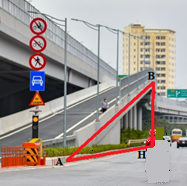
\includegraphics[scale=0.7]{images/1-B23-TLN-C5}
	}
	\loigiai{
		Khoảng cách từ mặt đường đến cầu vượt là $BH=AB\cdot \sin 30^\circ=6$ m.\\
		Vậy những phương tiện tham gia giao thông chiều cao phải nhỏ hơn $6$ mét.
	}
\end{ex}
\begin{ex}%[1H3B3-3]
Cho hình chóp $S.ABCD$ có đáy $ABCD$ là hình thang vuông tại $A$ và $B$, $AB=BC=a$, $AD=2a$. Cạnh bên $SA=a\sqrt{2}$ và vuông góc với đáy. Tính góc (đơn vị độ) giữa đường thẳng $SC$ với mặt phẳng $\left(SAD\right)$.\\
\shortans[oly]{$30$}
	\loigiai{
		\immini{
			Gọi $M$ là trung điểm $AD$, suy ra $ABCM$ là hình vuông nên $CM\perp AD$.\\
			Ta có $\heva{& CM\perp AD \\ & CM\perp SA \\}\Rightarrow CM\perp \left(SAD\right)$.\\
			Suy ra hình chiếu vuông góc của $SC$ trên mặt phẳng $\left(SAD\right)$ là $SM$.\\
			Do đó $\left( SC,\left(SAD\right)\right)=(SC,SM)=\widehat{CSM}$.\\
			Tam giác vuông $SMC$, có $$\tan \widehat{CSM}=\dfrac{CM}{SM}=\dfrac{AB}{\sqrt{SA^2+AM^2}}=\dfrac{1}{\sqrt{3}}\Rightarrow \widehat{CSM}=30^\circ.$$
		}{
			\begin{tikzpicture}[scale=0.7, font=\footnotesize, line join=round, line cap=round,>=stealth]
				\tkzDefPoints{0/0/B, 6/0/I, 8/2/D}
				\coordinate (A) at ($(B)+(D)-(I)$);
				\coordinate (S) at ($(A)+(0,5)$);
				\coordinate (M) at ($(A)!.5!(D)$);
				\coordinate (C) at ($(I)!.5!(B)$);
				\tkzDrawPoints[fill=black](A,B,C,D,S,M)
				\tkzDrawSegments[dashed](A,C S,A A,B A,D C,M S,M)
				\tkzDrawPolygon(S,B,C,D)
				\tkzDrawSegments(S,C)
				\tkzLabelPoints[above left](A)
				\tkzLabelPoints[above](S)
				\tkzLabelPoints[above right](M)
				\tkzLabelPoints[below](B,C)
				\tkzLabelPoints[above right](D)
				\tkzMarkRightAngles(S,A,D)
				\tkzMarkAngles[size=0.9](C,S,M)
			\end{tikzpicture}
		}
	}
\end{ex}

\begin{ex}%[1H3B3-3]
	Cho lăng trụ $ABCD.A'B'C'D'$ có đáy là hình thoi cạnh $a$, $\widehat{BAD}=60^\circ$. Hình chiếu vuông góc của $B'$ xuống mặt đáy trùng với giao điểm hai đường chéo của đáy và cạnh bên $BB'=a$. Tính góc (đơn vị độ) giữa cạnh bên và mặt đáy.\\
	\shortans[oly]{$60$}
	\loigiai{
		\immini{
			Gọi $O=AC\cap BD$. Theo giả thiết $B'O\perp \left(ABCD\right)$.\\
			Do đó $\left( BB',\left(ABCD\right)\right)=(BB',BO)=\widehat{B'BO}$.\\
			Vì tam giác $ABD$ đều cạnh $a$, suy ra $BO=\dfrac{1}{2}BD=\dfrac{a}{2}$.\\
			Tam giác vuông $B'BO$, có $$\cos \widehat{B'BO}=\dfrac{BO}{BB'}=\dfrac{1}{2}\Rightarrow \widehat{B'BO}=60^\circ. $$
		}{
			\begin{tikzpicture}[scale=0.7, font=\footnotesize, line join=round, line cap=round,>=stealth]
				\tkzDefPoints{0/0/D, 4/0/C, -2/-2/A}
				\coordinate (O) at ($(A)!.5!(C)$);
				\coordinate (H) at ($(O)!.5!(A)$);
				\coordinate (B) at ($(A)+(C)-(D)$);
				\coordinate (B') at ($(O)+(0,4)$);
				\tkzDefLine[parallel=through D](B,B') \tkzGetPoint{D'}
				\tkzDefLine[parallel=through C](B,B') \tkzGetPoint{C'}
				\tkzDefLine[parallel=through A](B,B') \tkzGetPoint{A'}
				\tkzDrawPolygon [dashed](D,C,A)
				\tkzDrawPolygon(A,B,C,C',D',A')
				\tkzDrawPoints[fill=black](A,B,C,D,O,A',B',C',D')
				\tkzDrawSegments[dashed](B,D O,B' D,D')
				\tkzDrawSegments(A,A' C',B' A',B' B,B')
				\tkzLabelPoints[above right](D)
				\tkzLabelPoints[below right](B')
				\tkzLabelPoints[right](C)
				\tkzLabelPoints[above](D',C',A')
				\tkzLabelPoints[below](A,B,O)
				\tkzMarkRightAngles(B,O,B')
				\tkzMarkAngles[size=0.9](B',B,O)
			\end{tikzpicture}
		}
	}
\end{ex}

\begin{ex}%[1H3B3-3]
	Cho hình hộp chữ nhật $ABCD.A'B'C'D'$ có đáy $ABCD$ là hình vuông cạnh bằng $2\sqrt{2}$, $AA'=4$. Tính góc giữa đường thẳng $A'C$ với mặt phẳng $\left(AA'B'B\right)$.\\
		\shortans[oly]{$30$}
	\loigiai{
		\immini{
			Ta có $\heva{& BC\perp AB \\ & BC\perp AA' \\}\Rightarrow BC\perp \left(AA'B'B\right)$.\\
			Do đó $\widehat{\left( A'C,\left(AA'B'B\right)\right)}=\widehat{\left(A'C,A'B\right)}=\widehat{CA'B}$.\\
			Vì $BC\perp \left(AA'B'B\right)$ $\Rightarrow BC\perp BA'$ nên tam giác $A'BC$ vuông tại $B$.\\
			Tam giác vuông $A'BC$, có $$\tan \widehat{CA'B}=\dfrac{BC}{A'B}=\dfrac{BC}{\sqrt{AA'^2+AB^2}}=\dfrac{1}{\sqrt{3}}.$$
			Vậy $A'C$ tạo với mặt phẳng $\left(AA'B'B\right)$ một góc $30^\circ$.
		}{
			\begin{tikzpicture}[scale=0.7, font=\footnotesize, line join=round, line cap=round,>=stealth]
				\tkzDefPoints{0/0/B, 6/0/C, 7.5/2/D}
				\coordinate (A) at ($(B)+(D)-(C)$);
				\coordinate (A') at ($(A)+(0,4)$);
				\coordinate (B') at ($(B)+(0,4)$);
				\coordinate (C') at ($(C)+(0,4)$);
				\coordinate (D') at ($(D)+(0,4)$);
				\tkzDrawSegments[dashed](A,A' A,D A,B A',B A',C)
				\tkzDrawPolygon(B,C,D,D',A',B')
				\tkzDrawSegments(C,C' B',C' C',D')
				\tkzDrawPoints[fill=black](A,B,C,D,A',B',C',D')
				\tkzLabelPoints[left](A)
				\tkzLabelPoints[above right](D)
				\tkzLabelPoints[above](A',B',C',D')
				\tkzLabelPoints[below](B,C)
				\tkzMarkAngles(B,A',C)
			\end{tikzpicture}
		}
	}
\end{ex}

\begin{ex}%[1H8V6-1]
	Cho hình chóp $S.ABCD$ có đáy $ABCD$ là hình chữ nhật tâm $O$, $AB=2a$, $AD=a\sqrt{2}$, $SA\perp(ABCD)$ và $SA=a\sqrt{3}$. Gọi $\alpha$ là góc giữa đường thẳng $SB$ và mặt phẳng $(SAC)$. Biết $\sin\alpha =\dfrac{2}{\sqrt{a}}$, tìm $a$.\\
	\shortans[oly]{$21$}
	\loigiai{
		\immini{Gọi $H$ là hình chiếu vuông góc của $B$ lên $AC$.\\
			Ta có $\heva{
				&BH\perp AC\\
				&BH\perp SA
			}$ $\Rightarrow$ $BH\perp(SAC)$ $\Rightarrow$ $SH$ là hình chiếu vuống góc của $SB$ lên $(SAC)$\\
			$\Rightarrow$ $\alpha =\left(\widehat{SB,(SAC)}\right)=\left(\widehat{SB,SH}\right)=\widehat{BSH}$.\\
			Ta có $SB=\sqrt{SA^2+AB^2}=a\sqrt{7}$ và\break $BH=\dfrac{AB. BC}{AC}=\dfrac{2\sqrt{3}}{3}a$.
		}
		{
			\begin{tikzpicture}[scale=1,>=stealth, font=\footnotesize, line join=round, line cap=round,declare function={h=2.5;}]
				\path
				(0,0) coordinate (A)
				(-1.3,-1.3) coordinate (B)
				(2.5,-1.3) coordinate (C)
				(barycentric cs:A=1,C=1,B=-1)coordinate(D)
				(barycentric cs:A=1,C=1)coordinate(O)
				(A)+(90:h) coordinate (S)
				(barycentric cs:A=4,C=1)coordinate(H)
				;
				\draw[dashed] (O)--(S)--(A)--(B)--(D)  (C)--(A)--(D) (S)--(H)--(B);
				\draw (C)--(S)--(B)--(C)--(D)--(S);
				\pic[draw,angle radius=5]{right angle=S--A--B};
				\pic[draw,angle radius=5]{right angle=S--A--C};
				\pic[draw,angle radius=5]{right angle=D--A--B};
				\pic[draw,angle radius=5]{right angle=B--H--O};
				\foreach \p/\g in{A/165,B/-90,C/-90,D/-45,S/90,O/-90,H/20}
				\fill[black](\p)circle(.03)node[shift={(\g:.3)},scale=1]{$\p$};
			\end{tikzpicture}
		}\noindent
		Xét tam giác $SBH$ vuông tại $H$ nên ta có $\sin\alpha =\dfrac{BH}{SB}=\dfrac{2}{\sqrt{21}}$ $\Rightarrow$ $a=21$.
	}
\end{ex}

\Closesolutionfile{ans}

